%-------------------------------------------------------------------------------
\chapter{Building and Integrating Estimators}
\labelchapter{ch.estimators}
%-------------------------------------------------------------------------------

%%%%%%%%%%%%%%%%%%%%%%%%%%%%%%%%%%%%%%%%%%%%%%%%%%%%%%%%%%%%%%%%%%%%%%%%%%%%%%%%
%%%%%%%%%%%%%%%%%%%%%%%%%%%%%%%%%%%%%%%%%%%%%%%%%%%%%%%%%%%%%%%%%%%%%%%%%%%%%%%%

\lettrine[lines=2]{T}{his} chapter discusses the definition of metrics used in hardware development processes, as well as their integration in a \myLongAc{HCF}{Hardware Construction Framework}.
We then consider different types of metrics to be used for hardware development, as well as various ways to estimate them, and finally expose a generic \myLongAc{API}{Application Programming Interface} for users to build their own estimation methodologies.

\vspace*{\fill}
\minitoc 
\mtcskip 

\newpage
%%%%%%%%%%%%%%%%%%%%%%%%%%%%%%%%%%%%%%%%%%%%%%%%%%%%%%%%%%%%%%%%%%%%%%%%%%%%%%%%

\section{Importance of Qualitative Estimations}
\label{ch.estimators:sec.estimators}
    In order to build efficient hardware designs under various constraints --- such as resource usage, power consumption or exploitable throughput --- hardware developers require quantitative estimations to make the best decision possible.
    However, design processes remain time-consuming tasks, and standard design methodologies rely on heavy computations --- \eg logic synthesis --- to obtain exploitable feedback, resulting in long turnaround times.
    In this section, we will consider different metrics and the quality of estimators to retrieve them, then discuss the importance of qualitative estimators for hardware design, and more specifically for \myLongAc{DSE}{Design Space Exploration}.

    \subsection{Quality of the Estimators}
    \label{ch.estimators:sec.estimators:ssec.quality}
        Various metrics can be used to define the quality of a hardware implementation, depending on the target circuit environment and the objectives of the developed accelerators.
        Among the most used metrics are resource usage, operating frequency, circuit latency or power consumption.
        However, they need to be adapted to the running environment of the design --- \eg resource usage can be defined as the area of silicon used when building \myLongAcs{ASIC}{Application-Specific Integrated Circuit}, but is most difficult to define for \myLongAc{FPGA}{Field-Programmable Gate Array} design, as multiple resources have to be considered due to the inherent heterogeneity of the boards (Fig. \ref{ch.problem:sec.hardware:ssec.fpga:sssec.fpga:fig.clb}).

        The quality of estimations needs to be considered to build efficient designs and exploration flows, as using poor estimators will more than probably result in a poor decision by the designer or by the exploration framework.
        However, we first need to define what is the quality of an estimator for a given metric, in order to quantify and compare multiple estimation techniques.
        Quality of an estimator can only be defined with respect to a reference value, \ie the expected value for the metric being estimated.
        In the rest of this work, we will consider {\bf synthesis results} as the reference value for both resource and frequency metrics, and consider estimators \myLongAc{QoR}{Quality of Results}\footnote{In the context of this thesis, both \myLongAc{QoR}{Quality of Results} and \myLongAc{QoS}{Quality of Service} notions will be used. Please refer to the glossary for disambiguation purposes.} with respect to vendor specific tools such as \tn{vivado} or \tn{Quartus}.

        In order to quantify quality estimators, we consider three aspects of an estimation methodology: {\bf accuracy}, {\bf faithfulness} and {\bf speed}.
        {\bf Accuracy} is defined as the proximity of the estimations to the expected values, while {\bf faithfulness} is defined using the standard deviation of the estimations --- \ie variation of estimators accuracy on different implementations.\footnote{Estimators \myAc{QoR} should thus consider both notions.}
        As a result, estimators can have high faithfulness but low accuracy --- \eg always estimating twice as many resources allows to easily compare different architectures, but can result in wrong design decisions as estimations are far from real values.
        Finally, {\bf speed} is defined with respect to the time needed to perform estimation.

        In this context, estimation methodologies offer different trade-offs between speed, accuracy and faithfulness, and estimator usage depends on the design goal.
        For example, to validate that a circuit is suitable for a given constraint set, one may consider slow but accurate estimations.
        Conversely, performing \myAc{DSE} requires fast and faithful estimators, but accuracy is not a main concern as the focus is put on comparing hardware implementations.

        We built Table \ref{ch.estimators:sec.estimators:ssec.quality:table.comparison} using our expertise and the literature introduced in Chapter \ref{ch.state}.
        It presents different estimation methodologies, as well as the corresponding quality metrics, showing different trade-offs depending on the usage.
        Standard \myLongAc{RTL}{Register-Transfer Level} methodologies are used as a baseline (Fig. \ref{ch.problem:sec.hardware:ssec.paradigms:fig.rtl}), since they are used to generate the reference values.
        Various works have explored rapid \myAc{RTL}-based estimations of both resource usage and operating frequency.
        However, critical paths are almost impossible to accurately estimate without running whole standard processes, therefore, \myAc{RTL}-based methodologies are not appropriate for such estimations.
        To cope with this challenge, \myLongAc{HLS}{High Level Synthesis} methodologies rely on fast resource estimations to allow quick exploration of the design space, but most tools use latency estimation and automatic scheduling rather than frequency estimation, in order to build accurate and controllable timing estimations.
        As for Spatial, it provides quick, reasonably faithful and accurate estimators, but the framework relies on a \myLongAc{DSL}{Domain Specific Language}, and is hence not adaptable to every possible use case.

        As a result, different metrics and estimation methodologies are to be considered for hardware development, depending on use case specificities --- this aspect is known as {\bf multi-fidelity metrics} usage and was already considered in the context of \myAc{HLS} exploration \cite{lo_multi-fidelity_2018}.

    \begin{table}[ht!]
        \centering
        \begin{adjustbox}{width=1.0\columnwidth,center}
            \begin{tabular}{c|ccccc}
                {\bf Entry level} & {\bf Metric} & {\bf Tools} & {\bf Accuracy} & {\bf Faithfulness} & {\bf Speed}\\
                \hline
                \multirow{2}*{RTL} & \ccg Resource, & \ccg Synthesis & \ccg & \ccg & \ccg \\
                ~ & \ccg frequency & \ccg (\tn{vivado}, \tn{Quartus}) & \ccg \multirow{-2}*{High} & \ccg \multirow{-2}*{High} & \ccg \multirow{-2}*{Slow}\\
                \multirow{2}*{RTL} & \multirow{2}*{Resource} & RTL estimation & \multirow{2}*{Low} & \multirow{2}*{Medium} & \multirow{2}*{Fast}\\
                ~ & ~ & \cite{schumacher_fast_2008}\cite{deng_accurate_2008} & ~ & ~ & ~\\
                \multirow{2}*{HLS} & \ccg Resource, & \ccg HLS tools & \ccg & \ccg & \ccg \\
                ~ & \ccg latency & \ccg \cite{canis2011legup}\cite{xilinx_vivado_2021} & \ccg \multirow{-2}*{Low} & \ccg \multirow{-2}*{Medium} & \ccg \multirow{-2}*{Fast}\\
                \multirow{2}*{DSL} & Resource, & \multirow{2}*{Spatial \cite{nardi_practical_2019}} & \multirow{2}*{Medium} & \multirow{2}*{Medium} & \multirow{2}*{Fast}\\
                ~ & frequency & ~ & ~ & ~ & ~\\
                \hline
            \end{tabular}
        \end{adjustbox}
        \caption[Estimation quality and abstraction level]{Comparison of different estimators depending on abstraction level}
        \label{ch.estimators:sec.estimators:ssec.quality:table.comparison}
    \end{table}

    \subsection{Feedback Usage for Hardware Development}
    \label{ch.estimators:sec.estimators:ssec.feedback}
        After defining qualitative concerns about metric estimators, we consider the different uses of metric estimation for hardware development processes.
        
        In standard \myAc{RTL} methodologies, iterating over produced designs is a time-consuming task as obtaining feedback about the developed circuit quality can take up to days of complex tool usage such as synthesis or place and route.
        To increase productivity, quick estimators can be used to swiftly provide feedback to developers, guiding them toward acceptable solutions while reducing the time spent in heavy computations --- however, significant time is still needed at the end of the process to validate that a design actually fits on the target board.
        
        Moreover, qualitative estimators are primordial for efficient \myAc{DSE}, as exploration speed is a main challenge for such methodologies --- actually, two levers can be considered to speed up exploration processes, namely exploration strategies and estimation methodologies.
        As exploration strategies will be considered in Chapter \ref{ch.dse}, this chapter will be dedicated to discussing the impact of estimation methodologies on \myAc{DSE} processes.

        As such processes are based on architecture comparisons in order to determine the impact of implementation options on resulting designs, one of the main challenges is related to how architectures should be compared.
        Thereupon, quick but faithful estimators need to be considered in such processes to perform meaningful comparisons in a reduced amount of time. 

%%%%%%%%%%%%%%%%%%%%%%%%%%%%%%%%%%%%%%%%%%%%%%%%%%%%%%%%%%%%%%%%%%%%%%%%%%%%%%%%

\section{Resource and Timing Estimations}
\label{ch.estimators:sec.resource-timing}

    Resource usage and timing concerns (\eg operating frequency, circuit latency) are among the principal considerations when it comes to \myAc{FPGA} development, as target specific constraints are to be respected for a design to pass the validation process.
    However, as stated in Section \ref{ch.estimators:sec.estimators}, classical flows used to produce such metrics are time consuming, resulting in long iterations over generated designs to find a suitable solution.

    This section hence considers building fast resource and timing estimators based on the \myLongAc{HCL}{Hardware Construction Language} paradigm to speed up its usage --- more specifically, we consider a \chisel{} based implementation.
    The aim is not to build state of the art estimators with particular focus on a good accuracy, but rather to integrate {\it proof of concept} estimators in an \myLongAc{HCF}{Hardware Construction Framework} and consider their usage as a way to increase hardware developer productivity.

    In order to do so, we chose to implement a resource estimation methodology similar to the one introduced by Schumacher \etal{} \cite{schumacher_fast_2008}, based on operator characterization and an \myLongAc{API}{Application Programming Interface} allowing users to model compilation steps that the synthesis tool is expected to take in order to provide realistic estimations.

    \subsection{Intermediate Representation Usage}
    \label{ch.estimators:sec.resource-timing:ssec.ir}

        Using \chisel{} as an entry point for a hardware development flow, one still requires a \myAc{HCF} to perform circuit elaboration, optimizations and backend emission, allowing the generated design to be fed to any \myAc{RTL} based toolchain.
        As an \myAc{HCF} requires an \myLongAc{IR}{Intermediate Representation} to operate on --- as does any compiler --- \myLongAc{FIRRTL}{Flexible Intermediate Representation for RTL} \cite{li_2016_specification}\cite{izraelevitz_2017_reusability} was introduced along \chisel{}.
        It was primarily built as an initiative to use \myAcs{HCL} for parametrized hardware library building, abstracting technology specific knowledge from the \myAc{HCF} frontend and relying on further transforms and backend to transform target-independent \myAc{RTL} to technology specific \myAc{RTL} --- allowing, for example, to use the same \chisel{} for both \myAc{ASIC} and \myAc{FPGA} targets.
        As a matter of fact, adapting software compilers structure --- \ie separating entry language (frontend), \myAc{IR} transforms and code generation (backend) --- enables to reuse \myAc{HCL} code, instead of using {\it ad-hoc} scripts to replace specific structures in the entry code to target a particular technology, as is usually done in standard development processes.
        Such target specific transforms can now be enabled by operating directly on the \myAc{IR}, and modifying the target technology becomes as simple as changing the transforms and configuration used for generation.
        Moreover, as both \chisel{} and \firrtl{} are based on \scala, high level programming features can be used for both hardware generator description and transform definition, enhancing developers expressivity for hardware description.

        Thereupon, to integrate estimators in an \myAc{HCF}, one must consider defining \myAc{IR} transforms as a way to operate on a given circuit and provide metric estimations in the process.

\clearpage
    \subsection{Basic Operator Characterization}
    \label{ch.estimators:sec.resource-timing:ssec.basic}

        Our first approach to build \firrtl{} based estimators is based on a naive approach of digital circuits, considering each operator individually on data paths, adding individual metrics to build global estimators.

        To begin with, we oppose costly \vs non costly operators --- based on our designer experience --- in Table \ref{ch.estimators:sec.resource-timing:ssec.basic:table.operator}, considering impact on both resource usage and data paths traversal time.

        \begin{table}[ht!]
            \centering
            \begin{adjustbox}{width=1.0\columnwidth,center}
                \begin{tabular}{c|ccc}
                    \multirow{2}*{{\bf Operator}} & \multirow{2}*{{\bf Description}} & \multirow{2}*{{\bf Impacting parameters}} & {\bf Considered}\\
                    ~ & ~ & ~ & {\bf for estimation}\\
                    \hline
                    {\tt ADD} & \ccg Adders & \ccg Operand widths & \ccg {\bf yes}\\
                    {\tt MULT} & Multipliers & Operand/result widths & {\bf yes}\\
                    \multirow{2}*{{\tt BINOP}} & \ccg Binary operations & \ccg ~ & \ccg ~\\
                    ~ & \ccg ({\tt OR}, {\tt AND}, {\tt NOT}, ...) & \multirow{-2}*{\ccg Operand widths} & \multirow{-2}*{\ccg {\bf yes}}\\
                    {\tt MUX} & Multiplexers & Operand/Condition widths & {\bf yes}\\
                    {\tt DSHIFT} & \ccg Dynamic shifts & \ccg Shift/result widths & \ccg {\bf yes}\\
                    {\tt REGISTER} & Registers & Element width & {\bf yes}\\
                    {\tt MEMORY} & \ccg Memory primitives & \ccg Memory width and depth & \ccg {\bf yes}\\
                    {\tt SSHIFT} & Static shifts & Input width & no\\
                    {\tt SELECT} & \ccg Bit selection among words & \ccg Result width & \ccg no\\
                    {\tt PAD} & Word padding & Result width & no\\
                    {\tt CAT} & \ccg Word concatenation & \ccg Result width & \ccg no\\
                    {\tt CONVERT} & Type conversion & Operand type and width & no\\
                    {\tt IO} & \ccg Input/output & \ccg Source/dest width & \ccg no\\
                    {\tt CONST} & Constant definition & Constant value & no\\
                    {\tt CONNECT} & \ccg Signal connection & \ccg Source/dest widths & \ccg no\\
                \end{tabular}
            \end{adjustbox}
            \caption[Operator impacts on estimations]{Operator impacts on both timing and resource usage estimations}
            \label{ch.estimators:sec.resource-timing:ssec.basic:table.operator}
        \end{table}

        To define non costly operators, we consider operations that are mostly reduced to rewiring of signals, as such action does not require particular resource usage but routing resources, and as wire traversal is considered non significant in this approach.% --- even if, for \myAc{FPGA} designs, Xu \etal{} \cite{xu_area_1996} up to 60\% of the critical path delay comes from routing.

        After identifying operators to consider for estimation, we use a pre-characterization based approach.
        To do so, we use vendor specific tools --- such as the \vivado{} synthesis tool for Xilinx \myAcs{FPGA} --- to generate {\bf reference values} for both resource usage and operator traversal time.
        Operators are characterized for a given set of different operand bit widths --- for example, adders are characterized with operands on 1, 2, 4, ..., 256 bits --- storing all the results in a {\bf library file} (using the \myAc{JSON} format).\footnote{Different operand widths are not considered in this process to enable single parameter characterization, thus only maximum operand bit width is considered for estimation in this naive approach.}
        Once this is done, we can use this characterized library to estimate both resource usage and timing of a given operator, using maximum operand bit width in the \firrtl{} representation as a parameter for estimation.
        The estimation process is then based on a simple statistical model: we retrieve the two nearest results --- \ie nearest maximum operand bit widths --- for an operator from the library, and estimate both resource usage and data path cost using linear regression between those two results, for each considered metrics.

        A first distinction is then to be made between resource and timing estimation: while we can estimate global resource usage by adding each individual operator estimation --- for each metric considered (\eg \myAcs{LUT}, \myAcs{FF}, \myAcs{DSP} and \myAcs{BRAM}) --- we need further circuit analysis to provide interesting timing estimations.

        \underline{Remark:} characterization is not mandatory for {\tt REGISTER} resource estimation as technological mapping is quite straightforward --- a n bit register will only use n \myAcs{FF}. 
        As for {\tt MEMORY} primitive estimations, both width and depth should be considered for estimation, and characterization is not needed either for the same reason.
        We thus use an {\it ad-hoc} computation of memory resource, based on a simple estimation of the total amount of bit in the {\tt MEMORY} primitive ($depth \times width$).

    \subsection{Data Path Building}
    \label{ch.estimators:sec.resource-timing:ssec.path}

        Timing considerations for hardware design are mainly based on the notion of {\bf critical path}.
        Critical path is defined as the longest path in the circuit --- each path corresponding to a sequence of wires and transistors from a starting point to an ending point, the longest being the one where the total traversal time is the greatest.
        In the context of synchronous designs, both starting and ending points are mostly defined as memory primitives, being either registers (\myAcs{FF}) or more complex memory components (\eg \myAcs{BRAM}).
        Circuit \myAcs{IO} are also to be considered for critical path definition, as they represent the interface with the external world, and may impact on the operating frequency.
        Maximal operating frequency is then defined as the inverse of the longest path traversal time, as operating at a higher frequency will result in some computation signals not being saved before new computations start.

        In order to provide a maximum operating frequency estimation based on \firrtl{}, we thus have to estimate traversal time of each possible path in the circuit, compare them, and expose the longest one(s) to users. 
        We consider three different cases in the process: register to register paths, \myAc{IO} to register paths, and register to \myAc{IO} paths. 
        It is important to note that the \firrtl{} representation uses a hierarchical approach for describing a circuit --- like do standard \myAcs{HDL} such as \verilog{} or \vhdl{} --- which is used to describe a complex circuit as a composition of simpler parts, the {\bf modules}.
        The main circuit of a design process is denoted as being the {\bf top level module}, and corresponds to the main \chisel{} class being compiled.
        One of the main challenges is hence to build every possible path, including {\bf cross-module} ones --- \ie paths originating in a module and terminating in another one --- which requires multiple passes over the circuit representation.

        Once every possible path is built, we can finally use individual operator traversal time estimations built in Section \ref{ch.estimators:sec.resource-timing:ssec.basic}.
        We consider a basic, addition based approach, where every estimation in a given path are added to estimate its total traversal time.
        We then compare each path traversal time, and provide users with feedback on timing concerns.

        \begin{figure}[h!]
            \centering
            \begin{subfigure}{1.0\textwidth}
                \centering
                \begin{adjustbox}{width=1.0\columnwidth,center}
                    \begin{tabular}{c|c|cccc|c}
                        {\bf Operator} & {\bf Bit width} & {\bf LUT} & {\bf FF} & {\bf DSP} & {\bf BRAM} & {\bf Path (ns)}\\
                        \hline
                        \multirow{3}*{{\tt ADD}} & \ccg 16 & \ccg 16 & \ccg 0 & \ccg 0 & \ccg 0 & \ccg 1.296\\
                        ~ & \ccg 32 & \ccg 32 & \ccg 0 & \ccg 0 & \ccg 0 & \ccg 1.512\\
                        ~ & \ccg 64 & \ccg 64 & \ccg 0 & \ccg 0 & \ccg 0 & \ccg 1.944\\
                        \multirow{3}*{{\tt MULT}} & 16 & 0 & 0 & 1 & 0 & 1.228\\
                        ~ & 32 & 0 & 0 & 4 & 0 & 4.176\\
                        ~ & 64 & 0 & 0 & 16 & 0 & 5.439\\
                        \multirow{3}*{{\tt REGISTER}} & \ccg 16 & \ccg 0 & \ccg 16 & \ccg 0 & \ccg 0 & \ccg 0.695\\
                        ~ & \ccg 32 & \ccg 0 & \ccg 32 & \ccg 0 & \ccg 0 & \ccg 0.695\\
                        ~ & \ccg 64 & \ccg 0 & \ccg 64 & \ccg 0 & \ccg 0 & \ccg 0.695\\
                    \end{tabular}
                \end{adjustbox}
                \caption{Characterized operator library for estimation (\Xilinx{} \VC{} board)}
                \label{ch.estimators:sec.resource-timing:ssec.basic:fig.estimation:sfig.lib}
                \vspace{1em}
            \end{subfigure}
            \begin{subfigure}{1.0\textwidth}
                \centering
                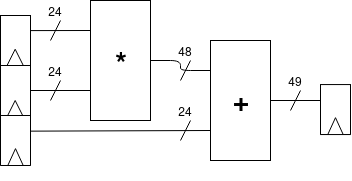
\includegraphics[width=0.65\textwidth]{Figures/Estimation-noMacro.png}
                \caption{Example of a simple circuit to estimate}
                \label{ch.estimators:sec.resource-timing:ssec.basic:fig.estimation:sfig.mac}
                \vspace{1em}
            \end{subfigure}
            \begin{subfigure}{1.0\textwidth}
                \centering
                \begin{adjustbox}{width=1.0\columnwidth,center}
                    \begin{tabular}{c|cc|cccc|c}
                        {\bf Operator} & {\bf \#} & {\bf Bit width} & {\bf LUT} & {\bf FF} & {\bf DSP} & {\bf BRAM} & {\bf Path (ns)}\\
                        \hline
                        {\tt ADD} & \ccg 1 & \ccg 32 & \ccg 32 & \ccg 0 & \ccg 0 & \ccg 0 & \ccg 1.512\\
                        {\tt MULT} & 1 & 24 & 0 & 0 & 3 & 0 & 2.702\\
                        {\tt REGISTER} & \ccg 3 & \ccg 24 & \ccg 0 & \ccg 24 & \ccg 0 & \ccg 0 & \ccg 0.695\\
                        {\tt REGISTER} & 1 & 49 & 0 & 49 & 0 & 0 & 0.695\\
                        \hline
                        {\bf Circuit} & ~ & ~ & 32 & 121 & 3 & 0 & 4.909 
                    \end{tabular}
                \end{adjustbox}
                \caption{Simple estimation of resource usage and critical path for a simple circuit (Fig. \ref{ch.estimators:sec.resource-timing:ssec.basic:fig.estimation:sfig.mac})}
                \label{ch.estimators:sec.resource-timing:ssec.basic:fig.estimation:sfig.results}
            \end{subfigure}
            \caption[Basic estimation methodology]{Basic estimation methodology based on individual characterization}
            \label{ch.estimators:sec.resource-timing:ssec.basic:fig.estimation}
        \end{figure}

        Figure \ref{ch.estimators:sec.resource-timing:ssec.basic:fig.estimation} introduces an example of this estimation methodology usage on a simple circuit (Fig. \ref{ch.estimators:sec.resource-timing:ssec.basic:fig.estimation:sfig.mac}), when targeting a \Xilinx{} \VC{} board.
        Sub results in Table \ref{ch.estimators:sec.resource-timing:ssec.basic:fig.estimation:sfig.results} are computed using characterized values from Table \ref{ch.estimators:sec.resource-timing:ssec.basic:fig.estimation:sfig.lib} and simple linear regression --- \eg for {\tt MULT} operator estimation on 24 bits, each value is computed using the average of values on both 16 and 32 bits.
        Then, for resource estimation, each individual estimation is added, while for critical path estimation, all paths are compared.
        
        In this case, critical path goes from a 24 bits register to the 49 bits register through both {\tt MULT} and {\tt ADD} operations, resulting in a total traversal time of $0.695 + 1.512 + 2.702 = 4.909$ ns\footnote{The {\tt REGISTER} traversal time is considered only once in the critical path.} --- corresponding to a maximum operating frequency of 204 MHz.


    \subsection{Limitations of the Approach}
    \label{ch.estimators:sec.resouce-timing:ssec.limitations}

        While this first approach for both resource and timing estimation is simple to apprehend, it presents some heavy limitations.

        First of all, the operators are estimated using only the maximum operand bit width as parameter.
        Nonetheless, some operators might require some additional parameters, as shown in Table \ref{ch.estimators:sec.resource-timing:ssec.basic:table.operator} --- such as {\tt MEMORY} primitives, {\tt MUXes} or {\tt DSHIFTs}.

        Moreover, the heterogeneous structure inherent to \myAcs{FPGA} led developers to consider specific design patterns, in order to take advantage of available resources on a given target.
        For example, \myLongAc{MAC}{Multiply and Accumulate} operations are commonly used in domains such as signal or image processing, and can use \myAcs{DSP} --- if available --- to favourably replace \myAcs{LUT} and improve performance while reserving resources for other computations.
        Such usage cannot be expressed when considering operators as individual entities, and higher granularity should be enabled in the flow.

        Finally, data paths can heavily differ depending on many factors such as the operation, the operands or the target.
        For instance, adders are usually implemented using {\bf carry adders}, each result bit being generated in a sequential way --- the first bit only requiring a 2 bit logical operation, while the n bit require every results in $[\![0, n-1]\!]$ to compute the input carry.
        Let $t_n$ be the traversal time of a n bit adder.
        We consider chaining two n bit adders $a_0$ and $a_1$, with the output of $a_0$ being one of the operand of $a_1$.
        Our naive approach consider the total traversal time of the path as being $2 \times t_n = t_{2\times n}$, however computations in $a_1$ can begin after only $t_1$, as computing $a_1$ first bit only requires knowledge about the first bit of $a_0$ result.
        This means that most of the total traversal time of this path is actually absorbed in a pipeline fashion, with a total traversal time of $t_{n+1}$ instead of $t_{2\times n}$.

        All of these properties must be considered in order to build exploitable estimators --- \ie estimators that may help designers into taking advantageous decisions in the development process --- as not considering them might result in erroneous feedback.

    \subsection{Macro Block Replacement}
    \label{ch.estimators:sec.resource-timing:ssec.macro}

        \begin{figure}[h!]
            \centering
            \begin{subfigure}{1.0\textwidth}
                \begin{adjustbox}{width=1.0\columnwidth,center}
                    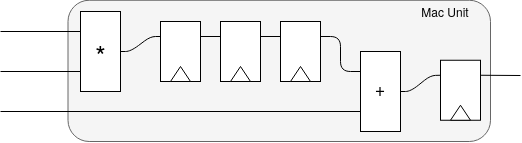
\includegraphics[width=1.0\textwidth]{Figures/MacroBlocks-Mac.png}
                \end{adjustbox}
                \caption{{\tt MAC} unit {\bf macro block} example for pattern $(R^3)(+^1)(R^1)$}
                \label{ch.estimators:sec.resource-timing:ssec.macro:fig.mac:sfig.pattern}
                \vspace{1em}
            \end{subfigure}
            \begin{subfigure}{1.0\textwidth}
                \begin{adjustbox}{width=1.0\columnwidth,center}
                    \begin{tabular}{c|c|cc}
                        {\bf Name} & {\bf Description} & {\bf Type} & {\bf Range}\\
                        \hline
                        \ccg {\it bit width} & \ccg maximum input bit width & \ccg generation & \ccg $[\![1, 256]\!]$\\
                        {\it outFactor} & useful output bit width & configuration & $[\![1, 2]\!]$\\
                        \ccg {\it mult register} & \ccg number of {\tt REGISTER} after {\tt MULT} & \ccg configuration & \ccg $[\![0, 3]\!]$\\
                        {\it add number} & number of {\tt ADD} in the {\tt MAC} pattern & configuration & $[\![0, 1]\!]$\\
                        \ccg {\it add register} & \ccg number of {\tt REGISTER} after {\tt ADD} & \ccg configuration & \ccg $[\![0, 1]\!]$
                    \end{tabular}
                \end{adjustbox}
                \caption{{\tt MAC} unit {\bf macro block} parameters w.r.t. \Xilinx{} \VC{} specifications}
                \label{ch.estimators:sec.resource-timing:ssec.macro:fig.mac:sfig.params}
            \end{subfigure}
            \caption[Multiply and accumulate macro block]{{\tt MAC} unit {\bf macro block}}
            \label{ch.estimators:sec.resource-timing:ssec.macro:fig.mac}
        \end{figure}
                
        \begin{figure}[h!]
            \centering
            \begin{subfigure}{0.85\textwidth}
                \begin{adjustbox}{width=0.5\columnwidth,center}
                    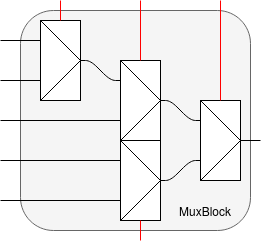
\includegraphics[width=1.0\textwidth]{Figures/MacroBlocks-MuxBlock.png}
                \end{adjustbox}
                \caption{{\tt MUXBLOCK} example with 5 inputs and 4 conditions}
                \label{ch.estimators:sec.resource-timing:ssec.macro:fig.mux:sfig.pattern}
                \vspace{1em}
            \end{subfigure}
            \begin{subfigure}{0.85\textwidth}
                \begin{adjustbox}{width=1.0\columnwidth,center}
                    \begin{tabular}{c|c|cc}
                        {\bf Name} & {\bf Description} & {\bf Type} & {\bf Range}\\
                        \hline
                        \ccg {\it bit width} & \ccg maximum input bit width & \ccg generation & \ccg $[\![1, 256]\!]$\\
                        {\it input number} & number of inputs & configuration & $2^{i, i \in [\![1, 8]\!]}$\\
                        \ccg {\it condition number} & \ccg number of conditions & \ccg configuration & \ccg $2^{i, i \in [\![0, 8]\!]}$\\
                    \end{tabular}
                \end{adjustbox}
                \caption{{\tt MUXBLOCK} parameters w.r.t. \Xilinx{} \VC{} specifications}
                \label{ch.estimators:sec.resource-timing:ssec.macro:fig.mux:sfig.params}
            \end{subfigure}
            \caption[Multiplexer macro block]{{\tt MUXBLOCK} {\bf macro block}}
            \label{ch.estimators:sec.resource-timing:ssec.macro:fig.mux}
        \end{figure}

        \begin{figure}[h!]
            \centering
            \begin{subfigure}{0.85\textwidth}
                \begin{adjustbox}{width=0.8\columnwidth,center}
                    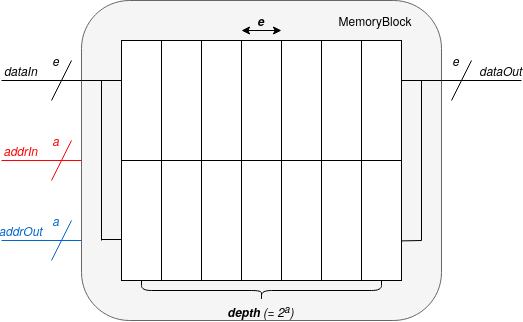
\includegraphics[width=1.0\textwidth]{Figures/MacroBlocks-MemoryBlock.png}
                \end{adjustbox}
                \caption{{\tt MEMORYBLOCK} schematic}
                \label{ch.estimators:sec.resource-timing:ssec.macro:fig.memory:sfig.pattern}
                \vspace{1em}
            \end{subfigure}
            \begin{subfigure}{0.85\textwidth}
                \begin{adjustbox}{width=1.0\columnwidth,center}
                    \begin{tabular}{c|c|cc}
                        {\bf Name} & {\bf Description} & {\bf Type} & {\bf Range}\\
                        \hline
                        \ccg {\it element width} & \ccg memory element bit width & \ccg generation & \ccg $[\![1, 1024$\\
                        {\it address number} & number of addresses & generation & $2^{i, i \in [\![1, 16]\!]}$\\
                        \ccg {\it register number} & \ccg number of register on address lines & \ccg configuration & \ccg $[\![0, 1]\!]$\\
                    \end{tabular}
                \end{adjustbox}
                \caption{{\tt MEMORYBLOCK} parameters w.r.t. \Xilinx{} \VC{} specifications}
                \label{ch.estimators:sec.resource-timing:ssec.macro:fig.memory:sfig.params}
            \end{subfigure}
            \caption[Memory macro block]{{\tt MEMORYBLOCK} {\bf macro block}}
            \label{ch.estimators:sec.resource-timing:ssec.macro:fig.memory}
        \end{figure}

        In order to improve this first approach, we now propose to consider more complex patterns for estimation, modelling steps that the synthesis tool is expected to take to pack operators \cite{schumacher_fast_2008}.
        To keep the method generic, we define two main steps for pattern recognition, replacement and estimation, and consider a user trying to find and replace $x$ different pattern $[\![p_0, ..., p_{x-1}]\!]$ in a \firrtl{} representation of a circuit.

        First of all, they need to define which pattern they are looking for, with respect to the \firrtl{} representation.
        To do so, we build a \myLongAc{DG}{Directed Graph} from a circuit \firrtl{} representation to operate on.
        We then developed a set of custom utility functions to scan the \myAc{DG}, recognize patterns and replace them by {\bf macro blocks} in the graph.
        We thus search and replace each pattern $p_{i, i \in [\![0, x-1]\!]}$ in the \myAc{DG} representation in a sequential fashion, therefore capturing complex computation patterns.
        At the end of the process, an updated \firrtl{} representation of the input circuit is produced in which all operators recognized as belonging to a particular {\bf macro block} are replaced by the corresponding {\bf macro block}.
        The \myAc{HCF} flow can then continue, and this representation can be fed into further \firrtl{} transforms --- \eg for estimation purposes.

        The second step is used to characterize the {\bf macro blocks} in a way similar to the one described in Section \ref{ch.estimators:sec.resource-timing:ssec.basic}.
        The user thus needs to provide a \chisel{} implementation generator for each pattern $p_{i, i \in [\![0, x-1]\!]}$, which is used to generate the {\bf reference values} for both resource usage and traversal time, using vendor tools such as \vivado{} syntheses.
        The generated values are then used to enhance the operator library with new parametrized {\bf macro blocks}.
        
        However, as stated in Section \ref{ch.estimators:sec.resource-timing:ssec.basic}, the first approach only considered single parameter estimation based on operator input bit width.
        To cope with such limitations, we consider two types of parameters to enhance the estimation process --- namely {\bf configuration parameters} and {\bf generation parameters}.
        The main difference between those two types is the value set width: {\bf configuration parameters} can be explored exhaustively for library building while {\bf generation parameters} would require too many runs and are thus only explored on a value subset for library building, before using linear regression for estimation as was done for bit widths in previous sections.
        Doing so enhances the library quality by adding a new entry for each possible configuration --- \ie each configuration in the cardinal product of {\bf configuration parameters} --- and each entry defines a regression based estimator for each considered metric (\myAc{LUT}, \myAc{FF}, \myAc{DSP}, \myAc{BRAM} and delay path), using {\bf generation parameters} as arguments of estimation functions.
        
        Three {\bf macro blocks} were considered to the enhanced basic operator library described in the first approach: \myLongAc{MAC}{Multiply and Accumulate} units, complex {\tt MUXBLOCK}s, and {\tt MEMORYBLOCK}s.
        Figure \ref{ch.estimators:sec.resource-timing:ssec.macro:fig.mac} introduces the {\tt MAC} unit macro blocks patterns and parameters, based on \Xilinx{} \VC{} specifications.
        This pattern is defined to fill \myAc{DSP} blocks with a maximum amount of \firrtl{} operations by packing them, in order to produce more accurate resource and timing estimations.
        This enables the {\tt MAC} patterns to absorb every {\tt MULT} operators and potential {\tt ADD}/{\tt REGISTER} operators in the same pattern, as the specifications state, for example, that \Xilinx{} \Virtex{} boards can absorb up to 4 {\tt REGISTER}s and one {\tt ADD} in a \myAc{DSP} block \cite{xilinx_dsp_2018}.
        Figure \ref{ch.estimators:sec.resource-timing:ssec.macro:fig.mux} presents a complex {\tt MUXBLOCK} macro block, as the \firrtl{} representation system only considers {\it 2-to-1} multiplexers in the emission process, resulting in erroneous estimations of {\it n-to-1} multiplexers, as they are represented as a chain of {\it 2-to-1} {\tt MUX} operations.
        In order to cope with those limitations, we thus absorb any {\tt MUX} pattern with {\it n} inputs and {\it m} conditions, and use {\bf macro block} characterization to improve resource estimation.
        Finally, {\tt MEMORYBLOCK} {\bf macro blocks} were introduced with respect to Table \ref{ch.estimators:sec.resource-timing:ssec.basic:table.operator}, as both element widths and depth must be considered for accurate estimation. 
        Figure \ref{ch.estimators:sec.resource-timing:ssec.macro:fig.memory} introduces both {\tt MEMORY} patterns and parameters, which are quite straightforward but enables a multi-variate estimation of the primitives using so defined characterized library methodology.

        \begin{figure}[ht!]
            \centering
            \begin{subfigure}{1.0\textwidth}
                \centering
                \begin{adjustbox}{width=1.0\columnwidth,center}
                    \begin{tabular}{c|c|cccc|c}
                        {\bf Operator/macro} & {\bf Bit width} & {\bf LUT} & {\bf FF} & {\bf DSP} & {\bf BRAM} & {\bf Path (ns)}\\
                        \hline
                        % \multirow{3}*{{\tt REGISTER}} & \ccg 16 & \ccg 0 & \ccg 16 & \ccg 0 & \ccg 0 & \ccg 0.695\\
                        % ~ & \ccg 32 & \ccg 0 & \ccg 32 & \ccg 0 & \ccg 0 & \ccg 0.695\\
                        % ~ & \ccg 64 & \ccg 0 & \ccg 64 & \ccg 0 & \ccg 0 & \ccg 0.695\\
                        \multirow{2}*{{\tt MAC} [2, 0, 1, 1]} & \ccg 16 & \ccg 0 & \ccg 0 & \ccg 1 & \ccg 0 & \ccg 1.000\\
                        ~ & 32 & 79 & 0 & 4 & 0 & 6.642\\
                    \end{tabular}
                \end{adjustbox}
                \caption{Characterized macro library for estimation (\Xilinx{} \VC{} board)}
                \label{ch.estimators:sec.resource-timing:ssec.macro:fig.estimation:sfig.lib}
                \vspace{1em}
            \end{subfigure}
            \begin{subfigure}{1.0\textwidth}
                \centering
                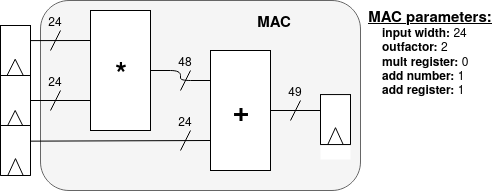
\includegraphics[width=0.7\textwidth]{Figures/Estimation-macro.png}
                \caption{Updated circuit from Figure \ref{ch.estimators:sec.resource-timing:ssec.basic:fig.estimation:sfig.mac} after macro recognition}
                \label{ch.estimators:sec.resource-timing:ssec.macro:fig.estimation:sfig.mac}
                \vspace{1em}
            \end{subfigure}
            \begin{subfigure}{1.0\textwidth}
                \centering
                \begin{adjustbox}{width=1.0\columnwidth,center}
                    \begin{tabular}{c|cc|cccc|c}
                        {\bf Operator/macro} & {\bf \#} & {\bf bit width} & {\bf LUT} & {\bf FF} & {\bf DSP} & {\bf BRAM} & {\bf Path (ns)}\\
                        \hline
                        {\tt MAC} [2, 0, 1, 1] & \ccg 1 & \ccg 24 & \ccg 40 & \ccg 0 & \ccg 3 & \ccg 0 & \ccg 3.821\\
                        {\tt REGISTER} & 3 & 24 & 0 & 24 & 0 & 0 & 0.695\\
                        \hline
                        {\bf Circuit} & \ccg ~ & \ccg ~ & \ccg 40 & \ccg 72 & \ccg 3 & \ccg 0 & \ccg 4.516\\
                    \end{tabular}
                \end{adjustbox}
                \caption{Macro based estimation of resource usage and critical path for Fig. \ref{ch.estimators:sec.resource-timing:ssec.macro:fig.estimation:sfig.mac} circuit}
                \label{ch.estimators:sec.resource-timing:ssec.macro:fig.estimation:sfig.results}
            \end{subfigure}
            \caption{Macro block based estimation methodology}
            \label{ch.estimators:sec.resource-timing:ssec.macro:fig.estimation}
        \end{figure}


        Using the macro block replacement technique to improve our basic estimation methodology enables better estimations of complex patterns, and thus better estimations of \firrtl{} circuits on \myAc{FPGA}.
        Figure \ref{ch.estimators:sec.resource-timing:ssec.macro:fig.estimation} enhances the estimation methodology exposed in Figure \ref{ch.estimators:sec.resource-timing:ssec.basic:fig.estimation} with macro block recognition and replacement.
        As macro blocks are parametrized by both {\bf generation} and {\bf configuration parameters}, we denote with {\tt MACRO} [$p_0$, ..., $p_{n-1}$] a {\bf macro block} with $n$ {\bf configuration parameters} $p_{x, x \in [\![0, n-1]\!]}$ in Figures \ref{ch.estimators:sec.resource-timing:ssec.macro:fig.estimation:sfig.lib} and \ref{ch.estimators:sec.resource-timing:ssec.macro:fig.estimation:sfig.results}.
        For example, the {\tt MAC} [2, 0, 1, 1] pattern represents a {\tt MAC} unit with an {\it outFactor} of 2, no {\tt REGISTER} after the {\tt MULT} operation, one {\tt ADD} operation and one {\tt REGISTER} after the computation. 
        As we can see, for a maximum {\it input bit width} of 16 bits, the whole pattern can be absorbed in only one \myAc{DSP}, while it would have taken one \myAc{DSP}, 32 \myAcs{LUT} and 33 \myAcs{FF} for the same pattern using only basic operator characterization.
        For the pattern introduced in Figure \ref{ch.estimators:sec.resource-timing:ssec.macro:fig.estimation:sfig.mac}, the estimations thus differ depending on the used methodology.


%%%%%%%%%%%%%%%%%%%%%%%%%%%%%%%%%%%%%%%%%%%%%%%%%%%%%%%%%%%%%%%%%%%%%%%%%%%%%%%%

% I'm so sorry
\vspace{-0.15cm}
\section{Quality of Service Estimation}
\label{ch.estimators:sec.qos}
\vspace{-0.1cm}

    Both timing and resources are key concerns when building hardware designs that target \myAcs{FPGA}, and should be considered in every design process.
    However, additional metrics should also be considered in specific use cases, as stated in Chapter \ref{ch.state}, and estimation methodologies should allow to easily integrate new metrics in order to be as flexible as possible.

    To demonstrate such flexibility, we chose to consider the \myLongAc{QoS}{Quality of Service} of circuits in our methodology, to demonstrate how additional estimators can be built and used in hardware design processes alongside resource and timing estimations.
    \myAc{QoS} is a main concern when it comes to particular domains such as \myLongAc{AxC}{Approximate Computing} or signal processing systems, as applications often require guarantees about the maximum error that may be introduced by approximations through computations.
    For example, usage of fixed point representations instead of IEEE-754 floating point numbers enable efficient hardware acceleration with no dedicated \myLongAc{FPU}{Floating-Point Unit}, but results in divergences with respect to the software computational model --- which often uses floating point representations as \myAcs{CPU} embed dedicated \myAc{FPU}.
    It is thus necessary to analyse the error introduced by such changes in the data representation to insure that acceleration does not provide erroneous results, in particular for critical systems.

    \subsection{Taxonomy of the Estimation Approaches}
    \label{ch.estimators:sec.qos:ssec.taxonomy}
    
        In order to build flexible estimators, we define a taxonomy for estimation methodologies and apply it to \myAc{QoS} estimation in Figure \ref{ch.estimators:sec.qos:ssec.taxonomy:fig.taxonomy}.
        An estimation can either be based on an analytic formula, an empirical approach, or both --- \eg when adding two fixed point numbers, one can consider the maximum error that may be generated, provide a statistical distribution of the two operands to derive an error model, or take an empirical approach and estimate the error by running multiple simulations.
        Each solution should be considered in this methodology to enable users to leverage their knowledge about the application domain and the target specificities --- \eg by making the decision to use \myAcs{FPU} if any are available on the target board.

        \begin{figure}[h!]
            \centering
            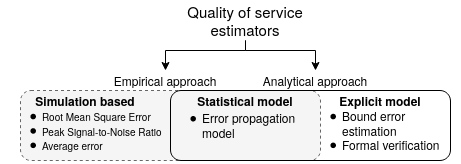
\includegraphics[width=1.0\textwidth]{Figures/taxonomy-qos.png}
            \caption{Taxonomy proposition for QoS estimators}
            \label{ch.estimators:sec.qos:ssec.taxonomy:fig.taxonomy}
        \end{figure}

    \subsection{Analytical Estimations}
    \label{ch.estimators:seq.qos:ssec.analytical}

        In order to provide analytical estimations for \myAc{QoS}, one should consider the specificities of both the data representation being used and the computations being performed.
        In most cases, a purely analytical approach is not desirable, as always considering the worst case for error propagation often results in inaccurate conclusions.
        For instance, knowing that an output on 8 bits with 4 bits of precision might have accumulated an error of $\pm 1/4$ does not bring any information on whether the implementation choices were good or not --- although can be used for critical system validation.
        Rather, statistical error propagation models can be used as basis to chose the data representation in a design, as assumptions on the statistical distributions of operands can help reduce the error propagation deduced from the analytical study of the system, and thus provide more relevant and exploitable results.

        In this context, we chose to enable users to define estimators at an analytical level, to derive \myAc{QoS} estimation from an expertise based analytical formula or error propagation models --- or any model based on analytical study of the design.
        Such estimators can use hardware generator parameters in analytical formulas, and should be achieved early in the flow, as they should not require further information about the circuit (see Section \ref{ch.estimators:sec.integration:ssec.multi-fidelity}).

    \subsection{Empirical Estimations}
    \label{ch.estimators:seq.qos:ssec.empirical}

        On the other hand, for non critical systems, an empirical approach may be used to provide \myAc{QoS} estimation, as occasional deviations for the expected behaviour should not have a noticeable impact on the design global \myAc{QoS} --- \eg occasional glitches in a video decoder are not as serious as erroneous results in the flight computer of plane.

\clearpage
        In this context, the users should be able to build estimators using simulation processes to bring information about empirical results.
        We thus integrate simulators in the estimation methodology, and propose helpers to build statistical analysis of empirical values to build significant estimators such as average error, standard deviation or \myLongAc{RMSE}{Root-Mean-Square Error} (which can be normalized).
        As a trade-off exists between the accuracy of an empirical estimator and the number of simulations to run, we expose the number of simulation runs as a parameter of the estimation process.

        After defining estimation methodologies for resource usage, critical paths and \myAc{QoS}, we then propose a generic way to integrate them in an \myAc{HCF}.

%%%%%%%%%%%%%%%%%%%%%%%%%%%%%%%%%%%%%%%%%%%%%%%%%%%%%%%%%%%%%%%%%%%%%%%%%%%%%%%%

\section[Integrating Metrics in a HCF]{Integrating Metrics in a Hardware\newline Construction Framework}
\label{ch.estimators:sec.integration}

    The main goal of this contribution is not to integrate a particular set of estimators to the chosen \myAc{HCF}, but rather to expose a generic \myAc{API} for users to define their own metrics and estimators with respect to their particular use cases.
    To do so, we propose a generic model for both metric definition and their integration in the framework, and apply them to the integration of estimators defined in Sections \ref{ch.estimators:sec.resource-timing} and \ref{ch.estimators:sec.qos}.

    \subsection{Exposing Multi-fidelity Estimators}
    \label{ch.estimators:sec.integration:ssec.multi-fidelity}
        In order to allow easy metric integration in the \chisel{} \myAc{HCF}, we start by defining abstraction levels where metric integration should be possible, as prior works exposed how {\bf multi-fidelity metrics} can be useful for exploration \cite{lo_multi-fidelity_2018} --- for it can enable either quick or accurate feedback depending on the needs and the exploration step.
    
        Figure \ref{ch.estimators:sec.integration:ssec.multi-fidelity:fig.flow} introduces the baseline \chisel{} development flow (Fig. \ref{ch.estimators:sec.integration:ssec.multi-fidelity:fig.flow:sfig.original}) and the proposed estimator integration steps (Fig. \ref{ch.estimators:sec.integration:ssec.multi-fidelity:fig.flow:sfig.proposed}).
        We choose to focus on three abstraction levels where estimators can be defined:
        \begin{itemize}
            \item Graph level --- \ie operating on \firrtl{} circuit representation
            \item Simulation level --- \ie using simulation results for estimation
            \item Register-Transfer level --- \ie calling \myAc{RTL} based external tools
        \end{itemize}

        As we can see on Figure \ref{ch.estimators:sec.integration:ssec.multi-fidelity:fig.flow:sfig.proposed}, the entry point of the flow is not altered with respect to the standard \chisel{} process (Fig. \ref{ch.estimators:sec.integration:ssec.multi-fidelity:fig.flow:sfig.original}).

\clearpage
        \begin{figure}[h!]
            \vspace{-0.1cm}
            \begin{subfigure}{0.49\textwidth}
                \centering
                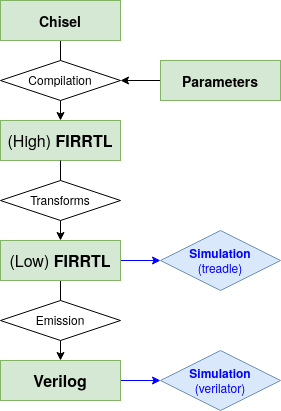
\includegraphics[width=0.75\textwidth]{Figures/chisel-flow-original.png}
                \vspace{3.5em}
                \caption{Chisel baseline development flow}
                \label{ch.estimators:sec.integration:ssec.multi-fidelity:fig.flow:sfig.original}
            \end{subfigure}
            ~
            \begin{subfigure}{0.49\textwidth}
                \centering
                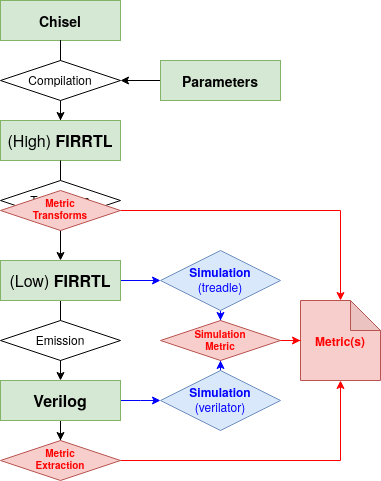
\includegraphics[width=1.0\textwidth]{Figures/chisel-flow-proposed.png}
                \caption{Integration of multi-fidelity metric in chisel development flow}
                \label{ch.estimators:sec.integration:ssec.multi-fidelity:fig.flow:sfig.proposed}
            \end{subfigure}
            \caption{Proposition for \chiselT{} flow enhancement}
            \label{ch.estimators:sec.integration:ssec.multi-fidelity:fig.flow}
            \vspace{-0.2cm}
        \end{figure}

        The {\bf graph level} estimators are then built by adding some custom transforms to the ones that are used by \chisel{} to produce a low \firrtl{} representation, while the {\bf simulation level} estimators are build by exposing an interface with the different {\bf simulation backends} that are integrated in \chisel{} and operate either at \firrtl{} level or on the generated \verilog.
        For readability purposes, we only expose the two main backends integrated in \chisel: \treadle{}, which is specific for \chisel{} and directly operate on the low \firrtl{} representation, and \verilator, which is an open-source tool that uses C++ for efficient cycle-accurate simulations.
        However, other simulators can be integrated as well, as long as they can be interfaced with one of the different representations at stake in the flow.
        Finally, the \myAc{RTL} estimators are integrated through the usage of the file system, and can rely on any tool that can take the generated \verilog{} descriptions as its entry points.

        Using those three abstraction levels, one can adjust both estimation \myAc{QoR} and speed for their custom flows in a generic way --- for example, both resource and timing estimators from Section \ref{ch.estimators:sec.resource-timing} are integrated at graph level, while \myAc{QoS} estimators from Section \ref{ch.estimators:sec.qos} are integrated either at simulation level or at graph level.
        The reference values that are computed through the syntheses are integrated at \myAc{RTL} level, showing that a classical design flow can also be achieved through this \myAc{API}.

\clearpage
    \subsection[Proposed Application Programming Interface]{Proposed {\it Application Programming Interface}}
    \label{ch.estimators:sec.integration:ssec.api}

        In order to integrate our estimation methodology in \chisel{} \myAc{HCF}, we propose to use the {\bf \firrtl{} transform system}, which is used by the framework to enable optimization and circuit generation through \myAc{IR} scans, as shown in Figure \ref{ch.estimators:sec.integration:ssec.multi-fidelity:fig.flow}.
        In fact, we define three levels for the integration:
        \begin{itemize}
            \item {\bf pre-elaboration} level --- which does not require \myAc{RTL} generation (\eg analytical approach)
            \item {\bf elaboration} level --- which operates on \firrtl{} representations (\eg resource and timing estimation)
            \item {\bf post-elaboration} level --- which operates after \myAc{RTL} generation (\eg simulation and syntheses)
        \end{itemize}
        
        {\bf Pre-elaboration} estimations are performed directly on the generator, by extracting metric estimations from constructor parameters, while {\bf post-elaboration} estimations are run at the end of the \myAc{HCF} process, and may leverage external tools such as synthesis suits or simulators.
        As for {\bf elaboration} estimators, they are integrated directly in the \firrtl{} flow, and uses the inner transform and annotation system --- which consists in a sequence of transforms operating on a circuit representation, which can modify it and/or use an annotation system to forward information in the flow --- to generate estimations from \myAc{IR} scans and forward it to the rest of the flow through annotation usage.

        At the end of an estimation run, all the estimated metrics can be collected from the annotation system, and used by the developers to iterate on their designs until a satisfying solution is found.

%%%%%%%%%%%%%%%%%%%%%%%%%%%%%%%%%%%%%%%%%%%%%%%%%%%%%%%%%%%%%%%%%%%%%%%%%%%%%%%%

\clearpage
\section[Synthesis on the Estimation Methodologies]{Synthesis on Estimation Methodologies}
\label{ch.estimators:seq.synthesis}

    In this chapter, we discussed the importance of qualitative estimations for hardware development processes, and put a particular focus on their application for \myLongAc{DSE}{Design Space Exploration}.

    We considered three different types of metric to be estimated --- namely resource usage, maximum operating frequency and \myAc{QoS} --- as well as how they can be estimated at different levels of fidelity.
    We proposed a simple estimation methodology based on an \myLongAc{IR}{Intermediate Representation} analysis for both spatial and temporal concerns, as well as an estimation taxonomy for \myLongAc{QoS}{Quality of Service} metrics, focusing on the \myLongAc{AxC}{Approximate Computing} domain.

    We then introduced a generic \myLongAc{API}{Application Programming Interface} integrated in the \chisel{} \myLongAc{HCF}{Hardware Construction Framework} to allow users to define their own metrics and estimators.
    This interface is supposed to be comprehensive enough to allow any user to leverage the \firrtl{} representation system to define their custom metrics.
    
    As the \myLongAc{QoR}{Quality of Results} of estimators is a main focus when it comes to \myAc{DSE}, various metrics and estimators will be considered in the next section, which will focus on building an exploration framework integrated in a \myAc{HCF}.

%%%%%%%%%%%%%%%%%%%%%%%%%%%%%%%%%%%%%%%%%%%%%%%%%%%%%%%%%%%%%%%%%%%%%%%%%%%%%%%%%
%%%%%%%%%%%%%%%%%%%%%%%%%%%%%%%%%%%%%%%%%%%%%%%%%%%%%%%%%%%%%%%%%%%%%%%%%%%%%%%
